\documentclass[a4j,dvipdfmx]{jsarticle}
\usepackage{graphicx}
%\usepackage{multirow}
%\usepackage{color}
%\usepackage{lscape}
%\usepackage{ascmac}
%\usepackage{txfonts}


\usepackage{listings, jlisting}
\renewcommand{\lstlistingname}{リスト}
\lstset{
  language={C},
  basicstyle=\ttfamily\scriptsize,
  commentstyle=\textit,
  classoffset=1,
  keywordstyle=\bfseries,
  frame=tRBl,
  framesep=5pt,
  showstringspaces=true,
  numbers=left,
  stepnumber=1,
  numberstyle=\tiny,
  tabsize=2
}


%% %subsubsubsectionの定義(できるだけ使わない方向で)
%% \makeatletter
%% \newcommand{\subsubsubsection}{\@startsection{paragraph}{4}{\z@}%
%%   {1.0\Cvs \@plus.5\Cdp \@minus.2\Cdp}%
%%   {.1\Cvs \@plus.3\Cdp}%
%%   {\reset@font\sffamily\normalsize}
%% }
\makeatother
\setcounter{secnumdepth}{4}
%ここまでsubsubsubsectionの定義

\begin{document}

\title{計算機科学実験及び演習4\\コンピュータグラフィックス\\課題3}
\author{工学部情報学科3回生 1029255242\\勝見久央}
\date{作成日: \today} % コンパイル時の日付が自動で挿入される
\maketitle
%文字コードはUTF-8推奨.それ以外ではline2のcontentsline~にエラー発生.
%選択範囲コメントアウトは選択中にM-;
%%%%%%%%%%%%%%%%%%%%%%%%%%%%%%%%%%%%%%%%%%%%%%%%%%%%%%%%%%%%%%%%%%%%%%
%ソースコードの貼付け
%% \lstinputlisting[caption=キャプション,label=ラベル,breaklines=true]
%% {./kadai01.sc}
%%次でも可
%% \begin{lstlisting}
%% \end{lstlisting}
\section{概要}
本実験課題では、3Dポリゴンデータを透視投影によって投影したPPM画像を生成する
プログラムを、課題2のプログラムkadai02.cを拡張させる形でC言語で作成した.
したがって、基本的な仕様は前回のReportForKadai02.pdfに準拠し、
本文では変更点に焦点を当てて言及することとする.

\section{要求仕様}
作成したプログラムが満たす仕様は以下の通りである.
\begin{itemize}
\item ポリゴンデータはVRML形式(拡張子wrl)のファイルで取り込む形式とした.
\item 光源方向は(x,y,z) = (-1.0, -1.0, 2.0)とした.
\item 光源の明るさは(r,g,b) = (1.0, 1.0, 1.0)とした.
\item 光源モデルは平行光源を採用した.
\item カメラ位置は(x,y,z) = (0.0, 0.0, 0.0)とした.
\item カメラ方向は(x,y,z) = (0.0, 0.0, 1.0)とした.
\item カメラ焦点距離は256.0とした.
\item ポリゴンには拡散反射に加えて鏡面反射を施した.
\item コンスタントシェーディングによりポリゴンを描画した.
\item zバッファによる隠面処理を行った.
\end{itemize}

\section{プログラムの仕様}
\subsection{留意点}
本課題では課題2と同様VRMLファイルの読み込みに与えられた
ルーチンを使用した.なお、主な課題2からの変更点については次に示す.
%===========================
\begin{description}
\item[{\bf -ADDED!}]double shininess
\item[{\bf -ADDED!}]double specular\_color[3]
\item[{\bf -MODIFIED!}]main(int argc, char *argv[])
\item[{\bf -MODIFIED!}]void shading(double *a, double *b, double *c, double *n, double *A)
\item[{\bf -MODIFIED!}]main(int argc, char *argv[])
\end{description}
%===========================

%% deprecated
%% \lstinputlisting[caption=vrml.c,label=vrml.c,breaklines=true]
%%                 {./vrml.c}
                
%% \lstinputlisting[caption=vrml.h,label=vrml.h,breaklines=true]
%%                 {./vrml.h}

\subsection{各種定数}
プログラム内部で使用した重要な定数について以下に挙げておく.
%======================================================================
\subsubsection{ppm}
次の定数はppmファイル生成のための定数である.
kadai02.cと同一のものを使用した.
\begin{itemize}
\item MAGICNUM\\
  ppmファルのヘッダに記述する識別子. P3を使用.
  
\item WIDTH, HEIGHT, WIDTH\_STRING, HEIGHT\_STRING\\
  出力画像の幅、高さ. ともに256とする. STRINGは文字列として使用するためのマクロ.
  以降も同様.
  
\item MAX, MAX\_STRING\\
  RGBの最大値. 255を使用.

\end{itemize}
%======================================================================
\subsubsection{環境設定}
次の定数は光源モデルなどの外部環境を特定する定数である.
\begin{itemize}
\item FOCUS\\
  カメラの焦点距離. 256.0と指定.
  
\item light\_dir[3]\\
  光源方向ベクトル.doubel型配列.
  
\item light\_rgb[3]\\
  光源の明るさを正規化したRGB値にして配列に格納したもの.
  double型配列.
  
\end{itemize}
%======================================================================
\subsubsection{その他}
\begin{itemize}
\item image[HEIGHT][WIDTH]\\
  描画した画像の各点の画素値を格納するための領域.
  領域確保のみで初期化は関数内で行う.
  double型の3次元配列.

\item z\_buf[HEIGHT][WIDTH]\\
  zバッファを格納するための領域.全ての頂点分のzバッファを格納する.
  初期化はmain関数内で行う.なお、初期化時の最大値としてはdouble型の最大値
  DBL\_MAXを使用した.
  double型2次元配列.
  
\item projected\_ver\_buf[3][2]\\
  ポリゴンを形成する3点に対して透視投影を施した結果の座標を保存しておくためのバッファ.
  なお、課題02で作成したkadai02.cの内部ではグローバル変数としていたが、
  kadai03.cではバグを避けるためmain内部で宣言する変数とした.
  double型2次元配列.
\item double shininess\\
  鏡面反射強度を格納するdouble型変数.
  
\item double specular\_color[3]\\
  鏡面反射係数を格納するdoubel型配列.
\end{itemize}

%======================================================================

\subsection{関数外部仕様}
\subsubsection{double func1(double *p, double *q, double y)}
kadai02.cと同一.
double型2次元配列で表された2点p、qの座標とdouble型の値yを引数に取り、
直線pqと直線y=yの交点のx座標をdouble型で返す関数.
ラスタライズの計算を簡素化するために三角形を分割する際に主に用いる.

\subsubsection{int lineOrNot(double *a, double *b, double *c)}
kadai02.cと同一.
double型2次元配列で表された3点a、b、cが一直線上にあるかどうかを判別する関数.
一直線上にある場合はint型1を返し、それ以外のときはint型0を返す.
後述の関数shadingの中で用いる.

\subsubsection{void shading(double *a, double *b, double *c, double *n, double *A)}
内部で変更があるが、外部仕様としてはkadai02.cと同一.
画像平面上に投影されたduble型2次元配列で与えられた3点a、b、cに対してシェーディングを行う関数.
%======================================================================================
\subsection{各関数のアルゴリズムの概要}
\subsubsection{double func1(double *p, double *q, double y)}
kadai02.cと同一.
2点p、qを通る直線の方程式を求めて、直線y=yとの交点を計算する.
なお直線pqがx軸に平行の時はエラーが発生する.

\subsubsection{int lineOrNot(double *a, double *b, double *c)}
kadai02.cと同一.
まず最初に3点a、b、cのx座標が全て同じであるかどうかを判定し、同じであれば一直線上にあると判定する.
同じでなければ、次に点cの座標を直線abの方程式に代入し、等号が成立するかどうかで一直線上に
あるかどうかを判定する。

\subsubsection{void shading(double *a, double *b, double *c, double *n)}
kadai02.cのものを拡張、変更した.
変更点は、ラスタ走査でシェーディングを行う際に、
描画中の点に対して鏡面反射を施すために必要な視線方向ベクトルを計算しながらシェーディングを行うという点である.
これは、テキストから抜粋した図\ref{fig:mirref}における、
\begin{figure}[htbp]
  \begin{center}
    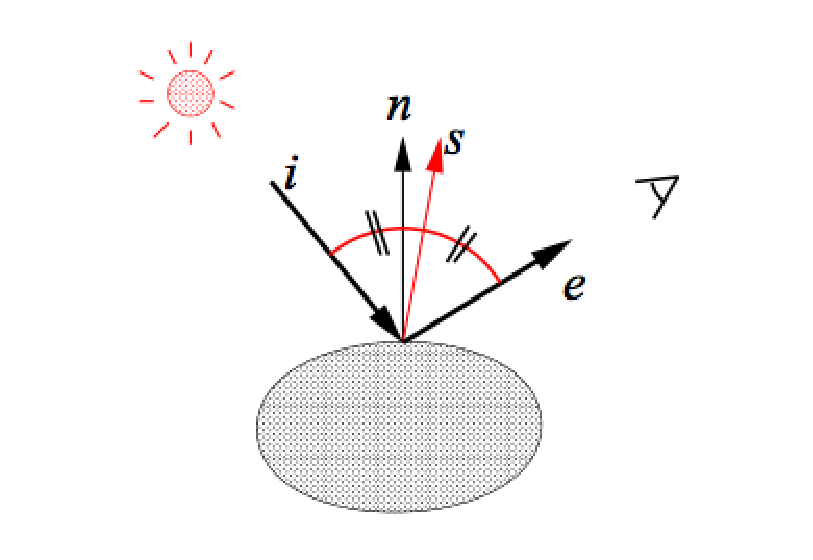
\includegraphics[clip,scale=0.5]{images/mirrorref.eps}
    \caption{鏡面反射(テキストより)}
  \end{center}
  \label{fig:mirref}
\end{figure}
ベクトルeを求める計算である. 
投影平面上の点$(x_{p}, y_{p})$の三次元空間内での座標は、カメラ位置(原点)と投影平面上の点を結ぶ直線と、
xyz空間内の元の三角形ABCを含む平面との交点を求める形で算出でき、元の三角形の法線ベクトルを
$(n_{x}, n_{y}, n_{z})$、点Aでの座標を$(x_{A}, y_{A}, z_{A})$、投影平面のz座標を$z_{p}$
とすると、
\begin{eqnarray}
(\frac{x_{p}(n_{x}x_{A}+n_{y}y_{A}+n_{z}z_{A})}{n_{x}x_{p} + n_{y}y_{p} + n_{z}z_{p}}, 
\frac{y_{p}(n_{x}x_{A}+n_{y}y_{A}+n_{z}z_{A})}{n_{x}x_{p} + n_{y}y_{p} + n_{z}z_{p}}, 
\frac{z_{p}(n_{x}x_{A}+n_{y}y_{A}+n_{z}z_{A})}{n_{x}x_{p} + n_{y}y_{p} + n_{z}z_{p}})
\end{eqnarray}
として表される.

\subsubsection{int main(int argc, char *argv[])}
kadai02.cのものを変更、拡張.
読み込むVRMLが記述されたファイル名(*.wrl)と
出力画像を書き込むppmファイル名(*.ppm)をコマンドライン引数として取得する.
kadai02.cからの変更点としては、main関数内部でグローバル領域に確保した鏡面反射係数を格納する配列と、
鏡面反射強度を格納する変数を初期化しする点である.
なお、鏡面反射強度についてはテキストの注意事項に記載のあった通り、VRMLに記載されている値を128倍して使用することとした.
\section{プログラム本体}
プログラム本体は次のようになった.
\lstinputlisting[caption=kadai03.c,label=kadai03.c,breaklines=true]{./kadai03.c}


\section{実行例}
kadai03.cと同一のディレクトリに次のプログラムを置き、
\lstinputlisting[caption=EvalKadai03.sh,label=EvalKadai03.sh,breaklines=true]{./EvalKadai03.sh}
さらに同一ディレクトリ内のディレクトリsampleの中に対象とするVRMLファイルを置いて、
\begin{lstlisting}
$ sh EvalKadai03.sh
\end{lstlisting}
を実行した.シェルスクリプト実行時に要求される引数で読み込むVRMLファイルを選択することができる.
出力画像は図\ref{fig:av4}、図\ref{fig:head}、図\ref{fig:1997}のようになった.

\begin{figure}[hp]
  \begin{center}
    
\includegraphics[clip,scale=0.5]{images/Kadai03ForAv4.eps}
    \caption{av4.wrlの出力結果}
    \label{fig:av4}
  \end{center}
\end{figure}


\begin{figure}[hp]
  \begin{center}
    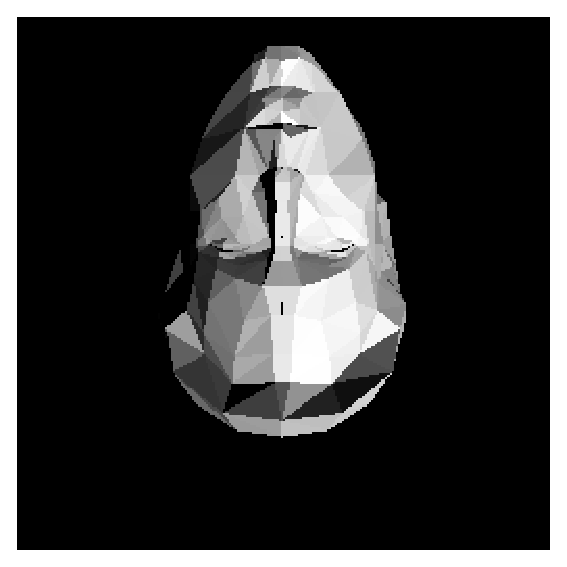
\includegraphics[clip,scale=0.5]{images/Kadai03ForHead.eps}
    \caption{head.wrlの出力結果}
    \label{fig:head}
  \end{center}
\end{figure}

\begin{figure}[hp]
  \begin{center}
    
\includegraphics[clip,scale=0.5]{images/Kadai03ForIiyama1997.eps}
    \caption{iiyama1997.wrlの出力結果}
    \label{fig:1997}
  \end{center}
\end{figure}

\section{工夫点、問題点、感想}
今回のプログラムでも本来は避けるべきグローバル領域に諸々の変数の格納領域を確保してしまっている.
しかしこの点について自分として少し考えた部分がある.
そもそもmain関数内にグローバル変数を置くことが懸念される最大の理由は、関数名のダブり及び予期しないグローバル変数の書き換えによるバグの発見の困難さである.
そのため、最初から初期化されている変数などについては、constを型宣言に加えてこれを防止するなどの処置がとられる.
しかしながら今回のプログラムではグローバル変数を多用している.
これは、このプログラムが完全に個人で作るものであるため、
自分だけが注意すれば変数名のダブりや意図しない書き換えについては防止できること、
グローバル変数として使用している変数を全て直接引数として関数呼び出しの際に与えると、
引数が多過ぎてプログラムの可読性が落ちるということ、さらには多数の引数分のメモリを
(z\_bufなどは殆どの場合要素数が$256 \times 256$個以上になる)
関数呼び出し、再帰呼出しの度にスタック領域に確保しなければならず、無駄が多いと考えたためである.
\section{APPENDIX}
ベースとしたkadai02.cのプログラムを付加しておく.
\lstinputlisting[caption=kadai02.c,label=kadai02.c,breaklines=true]{./kadai02.c}

\end{document}
